\begin{center}
	\textit{Stefano Di Vita, Gauthier Durieux, Christophe Grojean, Jiayin Gu, Zhen Liu, Giuliano Panico, Marc Riembau, Thibaud Vantalon}
\end{center} 

Assuming that the trilinear coupling is the only coupling deviating from its SM value, single Higgs observables can give competitive bounds with double Higgs production, see Refs.~\cite{Gorbahn:2016uoy,Degrassi:2016wml,Bizon:2016wgr,Degrassi:2017ucl,Maltoni:2017ims} \footnote{electroweak process where the Higgs trilinear coupling enter at the two loop level have also been studied in \cite{Kribs:2017znd}}. Nevertheless, departures of the Higgs self-coupling from its SM prediction signal the existence of new dynamics that, in general, would leave an imprint on other Higgs couplings as well which have a strong impact on the bound as shown by Ref.~\cite{DiVita:2017eyz}. The importance of a global fit is therefore two-fold, namely to assess the robustness of the studies that take into account deformations exclusively in the Higgs trilinear coupling, and to single out the sensitivity on the single-Higgs couplings that is required to minimize the impact of the possible correlations.
\medskip

\begin{figure}
	\centering
	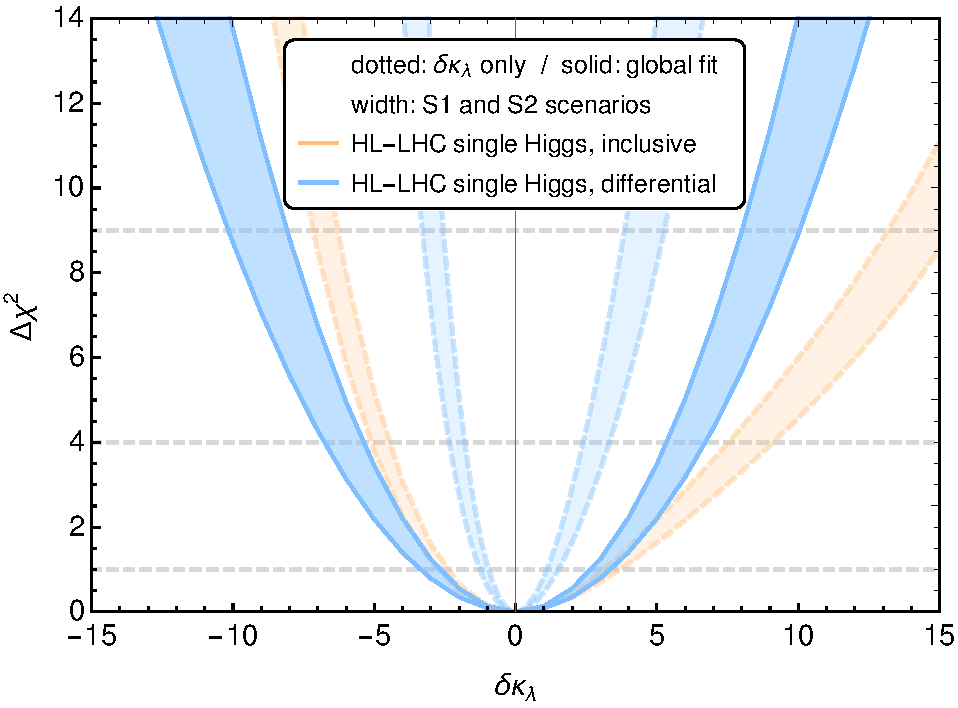
\includegraphics[width=0.45\linewidth]{\main/section3/plots/singlehHL}\hfill
	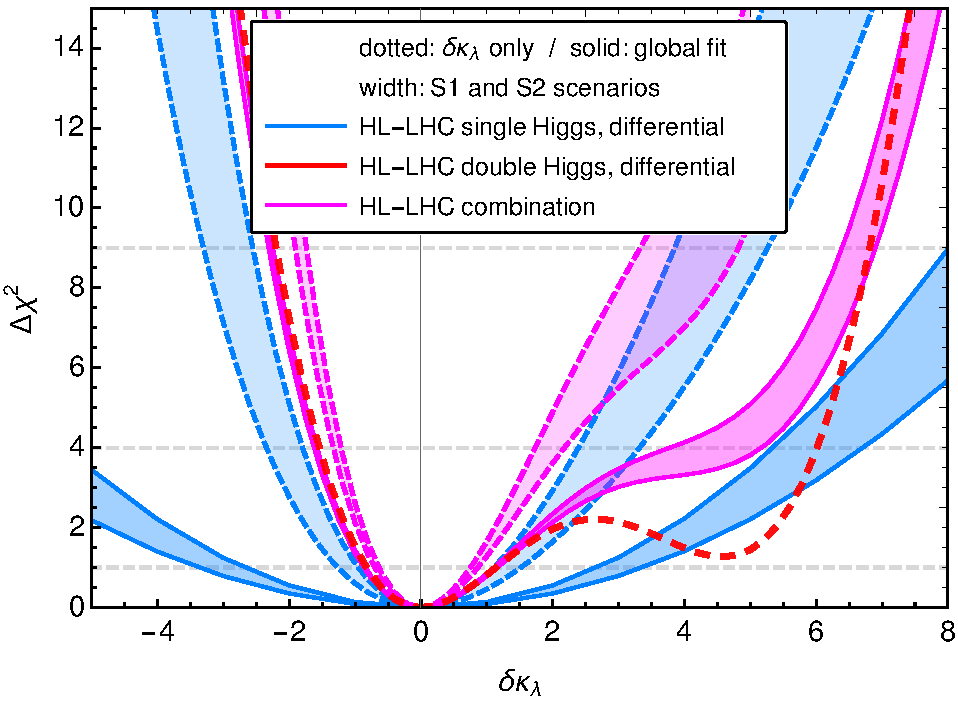
\includegraphics[width=0.45\linewidth]{\main/section3/plots/doublehhHL}
	\caption{$\chi^2$ analysis of the Higgs self-coupling $\delta \kappa_\lambda$ using single- and double-Higgs processes for the HL-LHC at 13\,TeV and 3\,ab$^{-1}$. The widths of the lines correspond to the differences between the scenarios S1 and S2. \textbf{Left:} Comparison of the constraints obtained using inclusive single-Higgs processes (orange), with the ones using differential observables (blue). Dashed is an exclusive fit while solid is the result of a global fit. \textbf{Right:} Comparison of the constraints from differential single Higgs (blue), with those from differential double-Higgs data (dashed red) and its combination (pink).}
	\label{fig:hllhcchi2}
\end{figure}

To include the effect of the different deformations away from the SM, we use the EFT framework described in Ref.~\cite{DiVita:2017eyz}, where 9 parameters describe the deviations of the single-Higgs couplings. In particular, we consider three\footnote{If other fermionic decay channels can be observed, further parameters can be included, with no effect on the number of degrees of freedom.} parameters for the Yukawa interactions ($\delta y_t,\,\delta y_b,\,\delta y_\tau,$), two for the contact interactions with gluons and photons ($c_{gg}\,,c_{\gamma\gamma}$), rescalings of the SM $hZZ$ and $hWW$ interactions (parametrized by one coefficient, $\delta c_z$, if custodial symmetry is unbroken), and three coefficients ($c_{zz},c_{z\square},c_{z\gamma}$) parametrizing interactions of the Higgs with the electroweak bosons that have non-SM tensor structures. Note that two combinations of the last three parameters are constrained by diboson data, showing an interesting interplay between the gauge and the Higgs sectors. A global fit on the Higgs self-coupling, parametrized by $\delta\kappa_\lambda$ (which is zero in the SM) using only inclusive single Higgs observables, and taking into account the additional 9 EFT deviations described above, suffers from a flat direction. To lift it, it is necessary to include data from differential measurements of those processes, since the single-Higgs deformations and $\delta\kappa_\lambda$ tend to affect the distributions in complementary ways.
\medskip

As input for the uncertainties we consider the S1 and S2 scenarios, corresponding to the projected uncertainties on the inclusive signal strengths of the different production and branching ratio modes of the Higgs, recommended by ATLAS and CMS. The projections of the differential uncertainties are estimated by first rescaling the statistical uncertainty on each bin. This gives an overestimation of the actual reach since it assumes a flat background distribution while it tends to peak at lower invariant masses. We use therefore the CMS analysis on $h\to \gamma \gamma$ in $t\bar{t} h$ production as a template for the tilt of the background. With this we get a good agreement with the CMS fit on the trilinear coupling using this channel only, and we use it as a simple guess for the rest of the uncertainties.
\medskip

The global fit for the HL-LHC is summarized in Fig.~\ref{fig:hllhcchi2}. In the left plot, we show in green the $\Delta\chi^2$ including only single-Higgs data, both in an exclusive study (dotted, pale color), and after profiling over all the other parameters (solid, strong color). The width of the lines correspond to the difference between the scenarios S1 and S2. The fact that the lines are not very separated means that the constraints are mostly statistics dominated. In orange, we consider only inclusive measurements, while in blue we include the differential information. We can see that, in a global fit, the constraint on the trilinear coupling is worsened due to correlations (mainly with the top yukawa $\delta y_t$ and the contact interaction with gluons $c_{gg}$, and, to a lesser degree, between $\delta y_b$ and $\delta c_z$. The inclusion of the differential information allows to partially remove the flat directions. In the right plot we compare the constraints using differential observables with the ones obtained from double Higgs production, taken from the study in Ref.~\cite{Azatov:2015oxa}, in dashed red. We include the combination in pink. While double-Higgs is clearly driving the bound, differential single-Higgs data is nonetheless relevant as it can help lift the degenerate minima around $\delta \kappa_\lambda\sim 5$.
\medskip

\begin{figure}
	\centering
	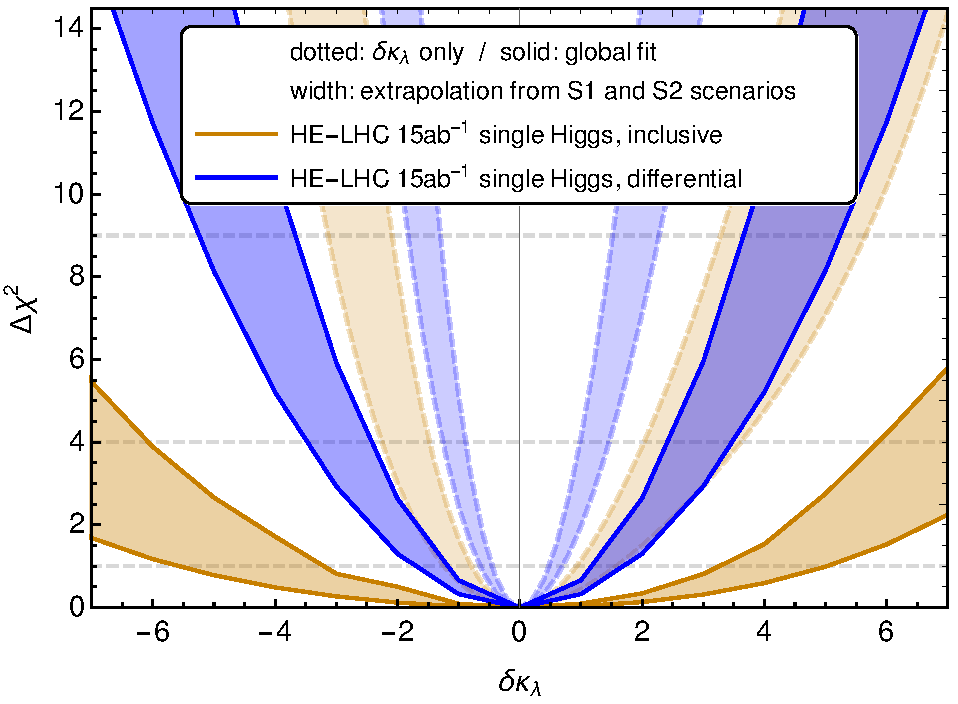
\includegraphics[width=0.45\linewidth]{\main/section3/plots/singlehHE}\hfill
	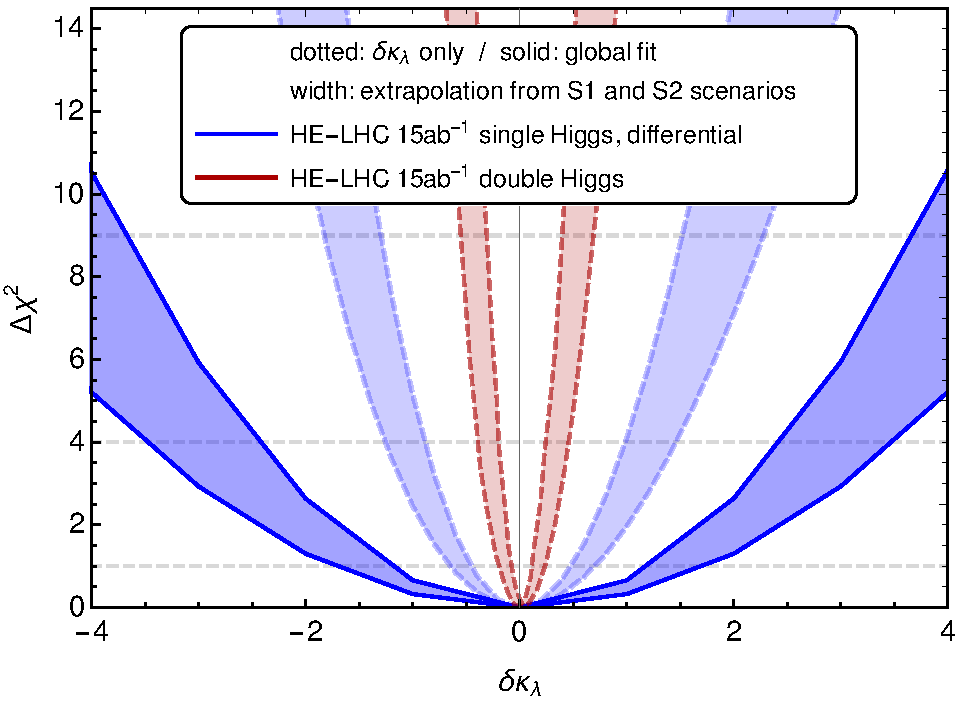
\includegraphics[width=0.45\linewidth]{\main/section3/plots/doublehhHE}
	\caption{$\chi^2$ analysis of the Higgs self-coupling $\delta \kappa_\lambda$ using single- and double-Higgs processes for the HE-LHC at 27\,TeV and 15\,ab$^{-1}$. The widths of the lines correspond to the differences between the projected uncertainties from the scenarios S1 and S2. \textbf{Left:} Comparison of the constraints obtained using inclusive single-Higgs processes (orange), with the ones using differential observables (blue). Dashed is an exclusive fit while solid is the result of a global fit. \textbf{Right:} Comparison of the constraints from differential single Higgs (blue), with those from differential double-Higgs data (dashed red).}
	\label{fig:helhcchi2}
\end{figure}	


We now discuss projections for the HE-LHC at 27\,TeV with 15\,ab$^{-1}$ of integrated luminosity. For the uncertainties we perform a simple extrapolation where the theory and systematic uncertainties are kept the same as in the HL-LHC projections, while the statistical uncertainty is rescaled accordingly \cite{Goncalves:2018qas}. We show the results in Fig.~\ref{fig:helhcchi2}. In the left plot, in brown, we present the $\chi^2$ analysis using the projections for the single-Higgs channels at HE-LHC at the inclusive level. Inclusive measurements are able to lift the flat direction due to the measurement of the $th+j$ production and the $z\gamma$ decay. In blue we present the results using differential observables. We note that the with of the line indicates that, contrary to the HL-LHC case, the constraint is limited by systematics, as expected. In the right plot we compare the constraints with the projections coming from double Higgs production measurement.
\medskip